% % % % % % % % % % % % % % % % % % % % % % % % % % % % % % % % % % % % % % % % % % % %
%                                                                                     %
% Short Sectioned Assignment LaTeX Template Version 1.0 (5/5/12)                      %
% This template has been downloaded from: http://www.LaTeXTemplates.com               %
%                                                                                     %
% Original author:  Frits Wenneker (http://www.howtotex.com)                          %
%                                                                                     %
% Modified by: Fco Javier Sueza Rodríguez (fcosueza@disroot.org)                      %
%                                                                                     %
% Changes:                                                                            %
%	    - Custom Chapters, Sections and Subsections (titlesec package)                %
%           - Document type scrbook (oneside)                                         %
%           - Use babel-lang-spanish package and marvosym                             %
%           - Use hyperref, enumitem, tcolorbox and glossaries packages               %
%           - Use Time New Roman (mathptmx), Helvetic and Courier fonts               %
%                                                                                     %
% License: CC BY-NC-SA 3.0 (http://creativecommons.org/licenses/by-nc-sa/3.0/)        %
%                                                                                     %
% % % % % % % % % % % % % % % % % % % % % % % % % % % % % % % % % % % % % % % % % % % %

%-----------------------------------------------%
%	              Packages                  %
%-----------------------------------------------%

\documentclass[paper=a4, fontsize=11pt, oneside]{scrbook}

% ---- Text Input/Output ----- %

\usepackage[T1]{fontenc}
\usepackage[utf8]{inputenc}
\usepackage{mathptmx}
\usepackage[scaled=.92]{helvet}
\usepackage{courier}
\usepackage[indent=12pt]{parskip}

\usepackage{geometry}
\geometry{verbose,tmargin=3cm,bmargin=3cm,lmargin=2.6cm,rmargin=2.6cm}

% ---- Language ----- %

\usepackage[spanish]{babel}
\usepackage{marvosym}

% ---- Another packages ---- %

\usepackage{amsmath,amsfonts,amsthm}
\usepackage{graphics,graphicx}
\usepackage{titlesec}
\usepackage{fancyhdr}
\usepackage{tcolorbox}
\usepackage{hyperref}
\usepackage{enumitem}
\usepackage[automake]{glossaries}

%--------------------------------------------------------------------%
%                      Customizing Document                          %
%--------------------------------------------------------------------%


% ----------- Custom Chapters, Sections and Subsections -------------- %

\titleformat{\chapter}[display]
			{\bfseries\Huge}
			{Tema \ \thechapter} {0.5ex}
			{\vspace{1ex}\centering}

\titleformat{\section}[hang]
			{\bfseries\Large}
			{\thesection}{0.5em}{}

\titleformat{\subsection}[hang]
			{\bfseries\large}
			{\thesubsection}{0.5em}{}

\titleformat{\subsubsection}[hang]
			{\bfseries\large}
			{\thesubsubsection}{0.5em}{}

\hypersetup{
    colorlinks=true,
    linkcolor=black,
    urlcolor=magenta
}

% ------------------- Custom heaaders and footers ------------------- %

\pagestyle{fancyplain}

\fancyhead[]{}
\fancyfoot[L]{}
\fancyfoot[C]{}
\fancyfoot[R]{\thepage}

\renewcommand{\headrulewidth}{0pt} % Remove header underlines
\renewcommand{\footrulewidth}{0pt} % Remove footer underlines

\setlength{\headheight}{13.6pt} % Customize the height of the header

% --------- Numbering equations, figures and tables ----------------- %

\numberwithin{equation}{section} % Number equations within sections
\numberwithin{figure}{section} % Number figures within sections
\numberwithin{table}{section} % Number tables within sections

% ------------------------ New Commands ----------------------------- %

\newcommand{\horrule}[1]{\rule{\linewidth}{#1}} % Create horizontal rule command


%----------------------------------------------------------------------------------------
%	TÍTULO Y DATOS DEL ALUMNO
%----------------------------------------------------------------------------------------

\title{
\normalfont \normalsize
\huge \textbf{Actividad Tarea 4}
}
\author{Francisco Javier Sueza Rodríguez}
\date{\normalsize\today}

%----------------------------------------------------------------------------------------
%                                     DOCUMENTO
%----------------------------------------------------------------------------------------
\begin{document}

\maketitle

\vspace{2ex}

\begin{center}
    \begin{tabular}{l l}
        \textbf{Centro}: & IES Aguadulce \\
        \textbf{Ciclo Formativo}: & Desarrollo Aplicaciones Web (Distancia)\\
        \textbf{Asignatura}: & Lenguajes de Marcas y Sistemas de Gestión de la Información\\
        \textbf{Tema}: & Tema 4 - Definición de Esquemas y Vocabulario en XML \\
    \end{tabular}
\end{center}

\vspace{10ex}

\section{Descripción}
Se van a responde a las preguntas sobre el enlazado de los documentos XML tanto con documentos dtd como xsd, relativas a la actividad 3 de la tarea 4.

\subsection{Preguntas sobre DTD}

\begin{itemize}
    \item ¿Qué modificaciones tendrías que hacer en el documento XML de ejemplo y en el documento DTD realizado en la actividad 1 para enlazar ambos archivos y poder validarlos?

    \textbf{Respuesta}:

    Para enlazar el documento XML con el DTD hay que añadir la cláusula \textbf{<!DOCTYPE>}, indicando en esta el nombre del elemento principal del documento, en este caso \textbf{envios}, si el documento es local o publico, en este caso es local por lo que se le añade la cadena \textbf{SYSTEM} y por último el nombre del fichero dtd. En nuestro caso, la clausula quedaría así:

    \begin{figure}[h]
        \begin{tcolorbox}[sharp corners, colback=yellow!30, colframe=white!20]
            \scriptsize
            \begin{verbatim}


                      <!DOCTYPE envios SYSTEM "envio.dtd">
            \end{verbatim}
        \end{tcolorbox}
    \end{figure}

    \item ¿Cómo los validarías con un editor especializado como NetBeans, u otro que valide este tipo de documentos?

    \textbf{Respuesta}:

    Depende un poco del IDE que se este empleando. En el casi de Netbeans, hay que pulsar el botón \textit{validar}, en el documento XML, para que se valide con el documento DTD enlazado. En otros IDEs como VSCode la validación se realiza cada vez que se modifica el documento.

    En la siguiente imagen, se muestra una validación correcta en Netbeans, es decir, que tras ejecutarse no muestra ningún error.

    \begin{figure}[H]
        \centering
        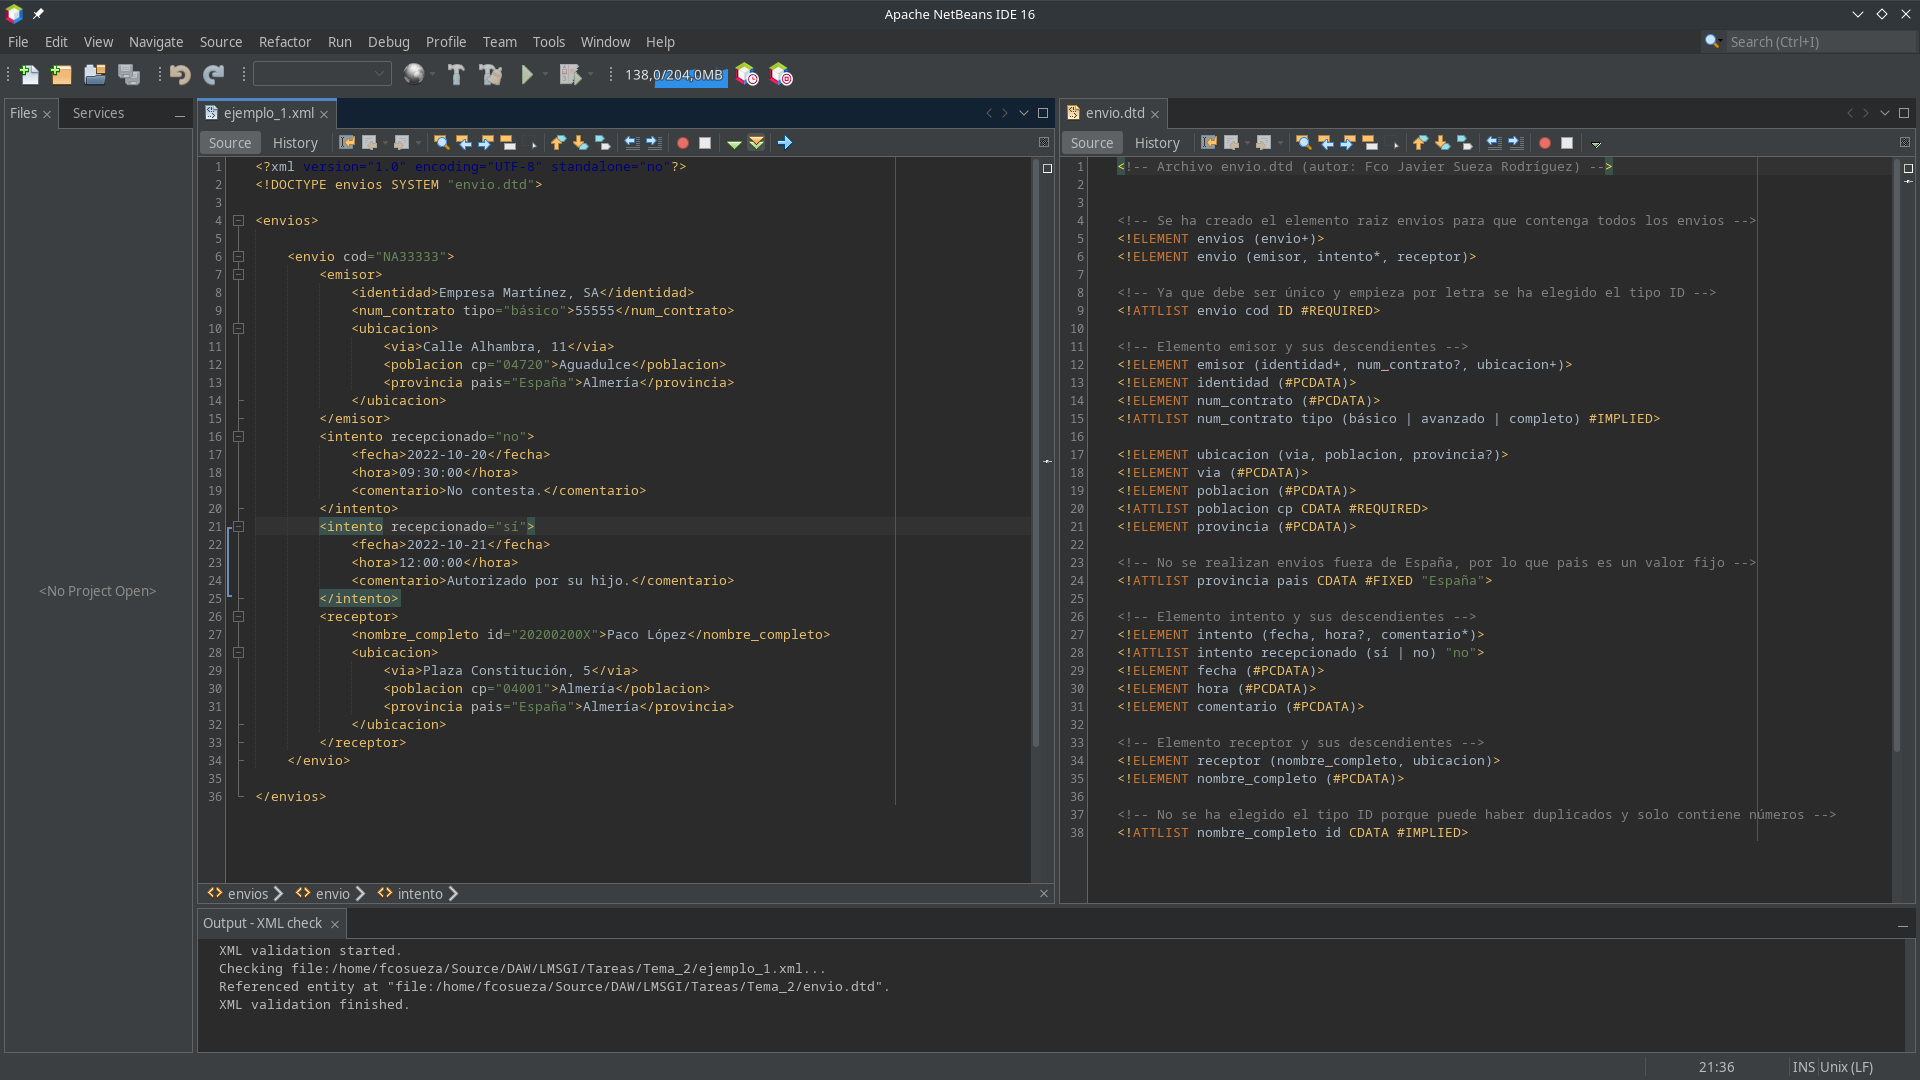
\includegraphics[scale=0.25]{validacion-dtd.png}
        \caption{Validación del XML con el DTD en Netbeans}
    \end{figure}
\end{itemize}

\subsection{Preguntas sobre XMl Schema}

\begin{itemize}
    \item ¿Qué modificaciones tendrías que hacer en el documento XML de ejemplo y en el documento XML Schema realizado en la actividad 2 para enlazar ambos archivos y poder validarlos?

    \textbf{Respuesta}:

    En el caso de XML Schema, el enlace del documento XML con el esquema se realizan mediante atributos en el elemento principal del XML. En este caso, hay que añadir los atributos \textbf{xmlns:xs} en el elemento envíos, el cual establece el espacio de nombres del esquema y lo fija al prefijo \textbf{xs}. Además, hay que indicar la ruta del archivo con el esquema, en este caso, añadiendo el atributo \textbf{xs:noNamespaceSchemaLocation} al elemento envíos.

    Como resultado, nuestro elemento \textbf{envíos} quedaría de la siguiente manera:

    \begin{figure}[h]
        \begin{tcolorbox}[sharp corners, colback=yellow!30, colframe=white!20]
            \tiny
            \begin{verbatim}
      <envios xmlns:xs="http://www.w3.org/2001/XMLSchema-instance"  xs:noNamespaceSchemaLocation="envio.xsd">
            \end{verbatim}
        \end{tcolorbox}
    \end{figure}

    \item ¿Cómo los validarías con un editor especializado como NetBeans, u otro que valide este tipo de documentos?

    \textbf{Respuesta}:

    Para la validarlo se hace de forma exactamente igual que con los archivos DTD, dependiendo también del IDE que se use. En nuestro caso hemos usado también Netbeans, como se puede ver en la siguiente imagen.

        \begin{figure}[H]
        \centering
        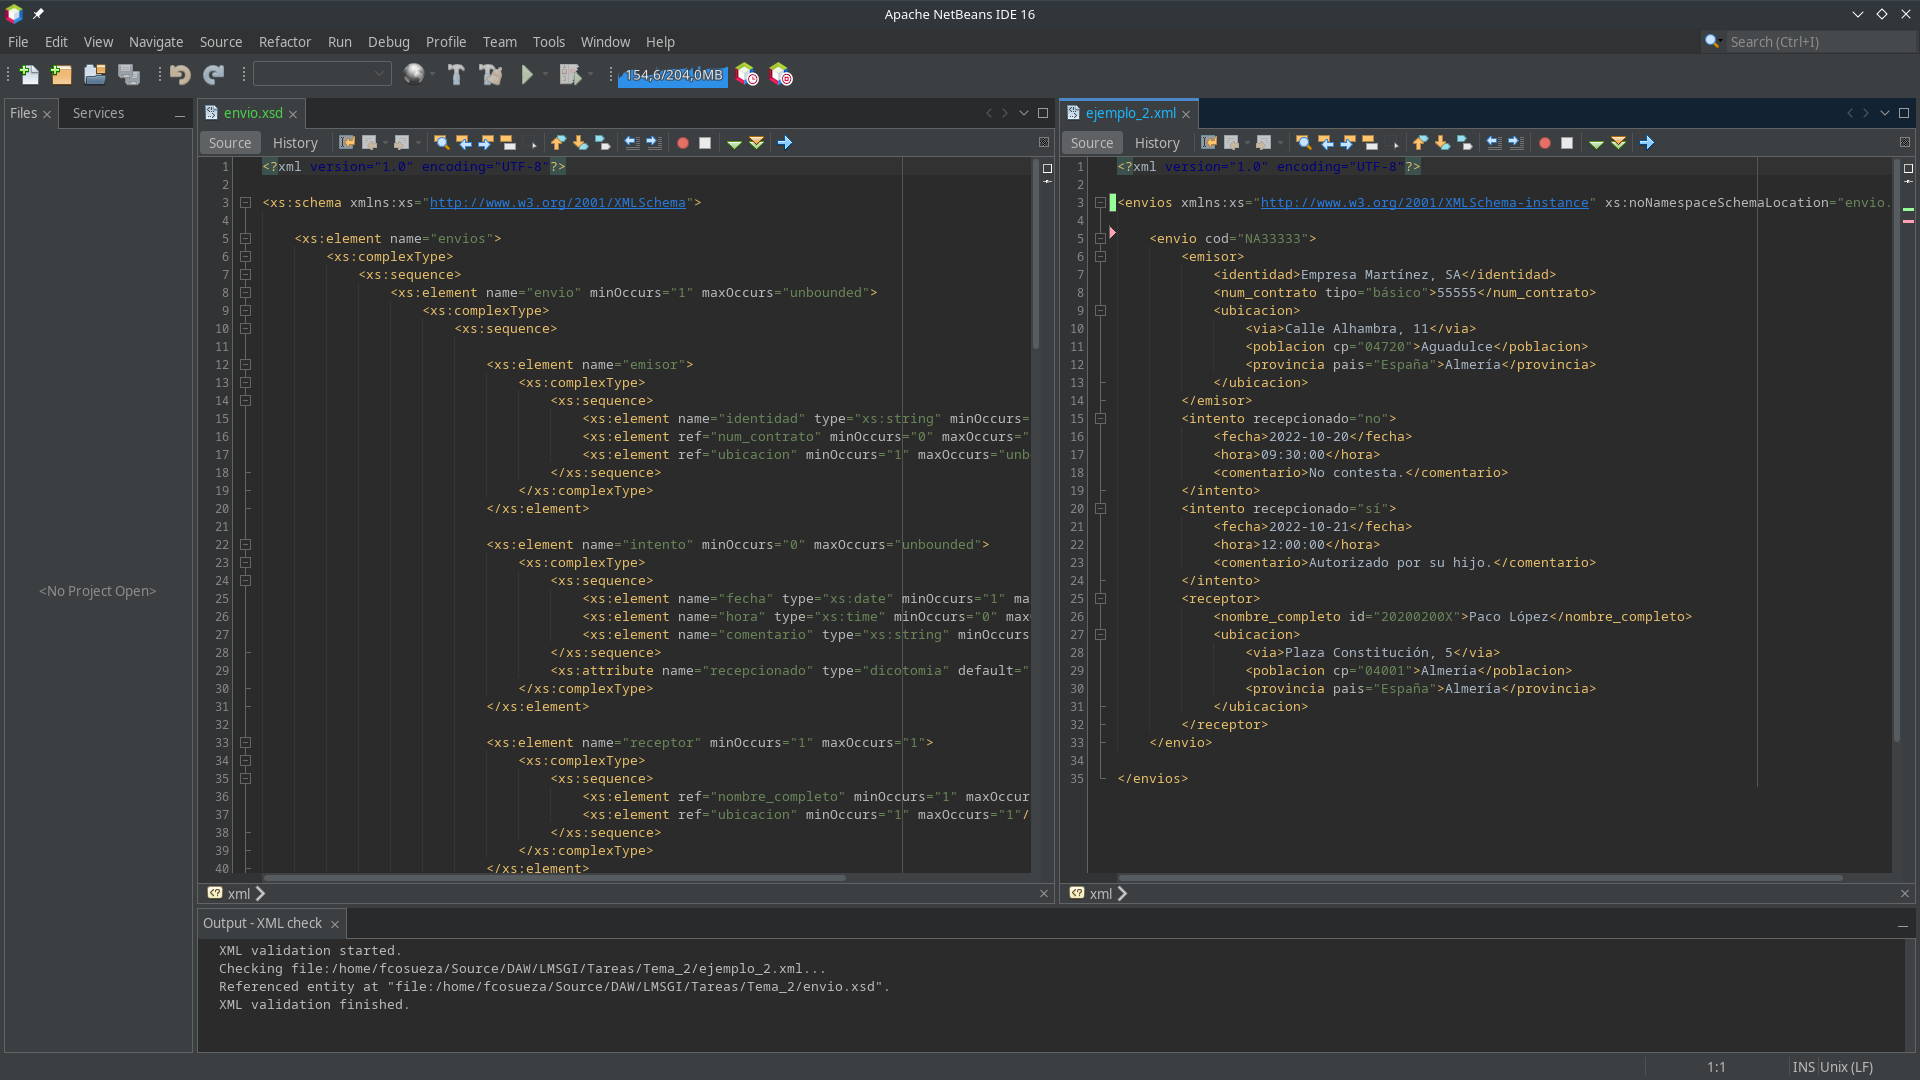
\includegraphics[scale=0.25]{validacion-xsd.png}
        \caption{Validación del XML con el XSD en Netbeans}
    \end{figure}
\end{itemize}

% Bibliography

%\newpage
%\bibliography{citas}
%\bibliographystyle{unsrt}

\end{document}